\documentclass[12pt, a4paper]{article}

\usepackage{amssymb}
\usepackage{multicol}
\usepackage{enumerate}
\usepackage[top=5em, bottom=5em, left=5em, right=5em]{geometry}
\usepackage{listings}
\usepackage{tikz}
\usetikzlibrary{positioning}

\setlength\parskip{1em}
\setlength\parindent{0em}

\title{Assignment 13}

\author{Hendrik Werner s4549775}

\begin{document}
\maketitle

This was done in collaboration with Constantin Blach (s4329872).

\section{} %1
\begin{enumerate}[(a)]
	\item %a
	It is proven that there exists a stable matching for any group size using the Gale–Shapley algorithm. We can just divide the people into two groups: Good and bad people. We then find a stable matching for both groups.

	Because a man eventually proposes to all women, everybody gets married in the end. Every woman that is proposed to will stick with the first proposer or switch him out later. In the end every woman is proposed to by some man so every woman is married which means that every man must also be married. (For every married woman there is a married man.)

	The marriages are stable because every man that prefers some woman over the one he gets at the end would have proposed to her earlier as she ranks higher than the woman he ended up with and got rejected.

	This means that there exists at least one stable matching where every good person is married to another good person and conversely ever bad person is married to another bad person.

	\item %b
	Every good person is ranked higher than every bad person. This means that every man will propose to all good women before he proposes to any bad woman. At the end every good woman is married to a good man because she rejects every bad man for any good man and all men propose to every good woman before proposing to any of the bad women. This means that at some point every good woman will be married to a good man because she will be proposed to by some good man (because he rather proposes to her than any of the bad women) at some point and reject any bad man she accepted earlier.

	After that there are only bad people left. We proved that there will exists a stable matching for the remaining people.

	In every stable matching all good people are married to another good person. This includes every good man being married to a good woman.
\end{enumerate}

\section{} %2

\section{} %3
The claim holds. An $n$ node simple graph $G$ is connected if every node has a degree of at least $n/2$.

Suppose we could split the graph into separate components that are not connected to each other. Each component has to contain at least $n/2 + 1$ nodes because we cannot connect to nodes outside of the component as that would break the component and each node has a degree of at least $n/2$. There are no self loops so the components needs at least $n/2$ other nodes any node in this component can connect to, which totals at least $n/2 + 1$.

We know the total number of nodes to be $n$. $\sum_{1 \leq k \leq c} (n/2 + 1) \leq n$, where $c$ is the number of components in the graph only holds for $c = 1$ so we know that there is only one component in the graph which means it is connected.

\section{} %4
\begin{enumerate}[(a)]
	\item %a
	Suppose $n = 2, M = 2$ and operating costs\\
	\begin{tabular}{|c||c|c|}
		\hline
		& Month 1 & Month 2\\
		\hline
		NY & 2 & 1\\
		\hline
		SF & 1 & 2\\
		\hline
	\end{tabular}

	The algorithm given produces $[SF, NY]$ with total operating costs of $4$.

	An optimal solution is $[NY, NY]$ with total operating costs of $3$.

	We have shown that the algorithm given does not produce plans with minimum cost.

	\item %b
	$n = 4, M = 0$ and operating costs\\
	\begin{tabular}{|c||c|c|c|c|}
		\hline
		& Month 1 & Month 2 & Month 3 & Month 4\\
		\hline
		NY & 1 & 0 & 1 & 0\\
		\hline
		SF & 0 & 1 & 0 & 1\\
		\hline
	\end{tabular}

	An optimal solution is $[SF, NY, SF, NY]$ which contains 3 moves.

	Every optimal plan must move at least 3 times because
	\begin{enumerate}
		\item there are 4 months,
		\item the moving cost is $M = 0$,
		\item and every month the operating cost is lower at another location compared to the previous month.
	\end{enumerate}

	\item %c
	You can find an optimal solution in $O(n)$.

	For every month beginning at month 1 you calculate the cost of staying there, and the cost of switching to the other location. You then return the minimum you found. This is done recursively.

	There is a lot of redundancy in the ensuing tree. Therefore you save every result you calculated and use them when they are needed again. This is the top down dynamic programming approach which dramatically cuts down on the time complexity.

	\paragraph{Correctness}
	The correctness proof is trivial: We exhaustively test the solution space and pick the best answer at each step. Because we consider all possibilities for each step and pick the optimal one the plan we get is also optimal.

	\paragraph{Time Complexity}
	We get a structure like this

	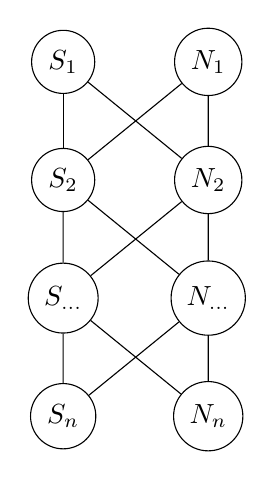
\begin{tikzpicture}[
		every node/.style={circle, draw, minimum width=2em}
		,baseline=(A.north)
	]
		\node (A) {$S_1$}
			child {
				node (B) {$S_2$}
				child {
					node (C) {$S_{\dots}$}
					child {
						node (D) {$S_n$}
					}
				}
			}
		;
		\node[right=of A] (H) {$N_1$}
			child {
				node (E) {$N_2$}
				child {
					node (F) {$N_{\dots}$}
					child {
						node (G) {$N_n$}
					}
				}
			}
		;

		\draw (A) edge (E);
		\draw (B) edge (F);
		\draw (C) edge (G);
		\draw (E) edge (C);
		\draw (F) edge (D);
		\draw (H) edge (B);
	\end{tikzpicture}

	where $N_i$ indicates that during month $i$ you should use the office in New York and $S_i$ indicates the same for San Francisco.

	The height of the tree is $n$ and therefore exploring the whole search space requires visiting $2n$ nodes and performing $O(1)$ work at each which totals $O(n)$.

	(This assumes that cache lookup is $O(1)$, using Hash Tables for example.)
\end{enumerate}

\end{document}
